%%%%%%%%%%%%%%%%%%%%%%%%%%%%%%%%%%%%%%%%%%%%%%%%%%%%%%%%%%%%%%%%%%%%%%%%%%%%%%%%
%2345678901234567890123456789012345678901234567890123456789012345678901234567890
%        1         2         3         4         5         6         7         8

\documentclass[letterpaper, 10 pt, conference]{ieeeconf}  % Comment this line out if you need a4paper

%\documentclass[a4paper, 10pt, conference]{ieeeconf}      % Use this line for a4 paper

\IEEEoverridecommandlockouts                              % This command is only needed if
                                                          % you want to use the \thanks command

\overrideIEEEmargins                                      % Needed to meet printer requirements.

% The following packages can be found on http:\\www.ctan.org
\usepackage{graphics} % for pdf, bitmapped graphics files
\usepackage{epsfig} % for postscript graphics files
\usepackage{mathptmx} % assumes new font selection scheme installed
\usepackage{times} % assumes new font selection scheme installed
\usepackage{amsmath} % assumes amsmath package installed
\usepackage{amssymb}  % assumes amsmath package installed
\usepackage{cite} % useful for handling multiple citations like \cite{a,b,c}
% TODO: Update your Title here
\title{\LARGE \bf
Overcoming Visual Clutter in Vision Language Action Models via Concept-Gated Visual Distillation
}

% TODO: Update your Authors here
\author{Sangmin Song$^{1}$, Sarath Kodagoda$^{1}$, Marc Carmichael$^{1}$ and Karthick Thiyagarajan$^{2}$% <-this % stops a space
\thanks{$^{1}$Sangmin Song, Sarath Kodagoda, and Marc Carmichael are with the University of Technology Sydney, NSW, Australia
        {\tt\small Sangmim.song@uts.edu.au }}%
\thanks{$^{2}$Karthick Thiyagarajan is with Western Sydney University, NSW, Australia
        {\tt\small K.Thiyagarajan@westernsydney.edu.au}}%
}

\begin{document}

\maketitle
\thispagestyle{empty}
\pagestyle{empty}

%%%%%%%%%%%%%%%%%%%%%%%%%%%%%%%%%%%%%%%%%%%%%%%%%%%%%%%%%%%%%%%%%%%%%%%%%%%%%%%%
\begin{abstract}
Vision-Language-Action (VLA) models demonstrate impressive zero-shot generalization but degrade sharply in cluttered scenes, a failure we term the ``Precision-Reasoning Gap'' and hypothesize to reflect background-induced feature dilution: semantically confusable clutter corrupting the visual grounding required for precise manipulation. We propose Concept-Gated Visual Distillation (CGVD), a training-free, model-agnostic inference-time framework that parses the instruction into safe and distractor sets, applies a two-layer target refinement---cross-validation and spatial disambiguation---that penalizes false positives, and removes the remaining distractor regions via image inpainting, preserving scene context outside the edited regions. Compared against the un-augmented $\pi_0$ and GR00T policies in SimplerEnv, CGVD substantially improves robustness to semantic clutter---on \textit{put spoon on towel} with 18 semantic distractors, $\pi_0$'s success rate rises from 43.0\% to 77.5\% (Table~\ref{tab:ablation})---and, under descriptive compositional prompts, to attribute clutter. At the same condition, a vocabulary-matched reimplementation of the run-time intervention baseline BYOVLA reaches 32.5\% at roughly $34\times$ CGVD's per-step cost. The protection is task- and distractor-type-conditional: on \textit{put carrot on plate}, where contextual clutter aids the baseline policies, CGVD provides no benefit at any tested density and often significantly underperforms them. Runtime compositing adds a measured ${\approx}16$\,ms (${+}5\%$) per control step after a one-off per-episode initialization of $0.7$--$3.3$\,s depending on scene complexity. These results support inference-time visual distillation as a practical defense against semantically confusable clutter for frozen VLA policies in static scenes.
\end{abstract}



\section{INTRODUCTION}


Vision-Language-Action (VLA) models~\cite{openvla, rt2, octo, gr00t, pi0} ground large language models into robotic control, enabling robots to follow open-vocabulary instructions like ``Put spoon on towel'' without task-specific training, and promising operation in unstructured, human-centric environments.

However, a significant gap remains between the semantic reasoning capabilities of these models and their geometric precision in deployment conditions. While VLAs excel in curated, clutter-free environments, their performance degrades precipitously in the presence of visual clutter~\cite{distracted_robot}, and more broadly under physical variations of the scene~\cite{eva_vla}. We term this phenomenon the Precision-Reasoning Gap: the model successfully identifies the target object conceptually, yet fails to manipulate it precisely. We hypothesize that attention corruption from surrounding distractors dilutes the latent representation used for spatial planning; under this hypothesis, feature dilution would manifest as high-variance trajectories, hesitation near distractors, and ultimately manipulation failure. Our experiments (\S\ref{sec:experiments}) measure the end-to-end effect of removing distractors; they do not directly instrument the attention mechanism, so we present this account as a working hypothesis rather than an established mechanism.

Critically, this degradation is not uniform across distractor types. We observe that failure concentrates around distractors sharing visual or semantic properties with the target, consistent with prior reports~\cite{distracted_robot}. While VLAs may exhibit resilience to arbitrary clutter via large-scale pre-training, they remain brittle to semantically confusable objects; for example, a fork scattered near a target spoon triggers conflicting visual tokens within the same affordance category, causing the policy to attend to or even grasp the wrong object.

\begin{figure*}[t]
    \centering
    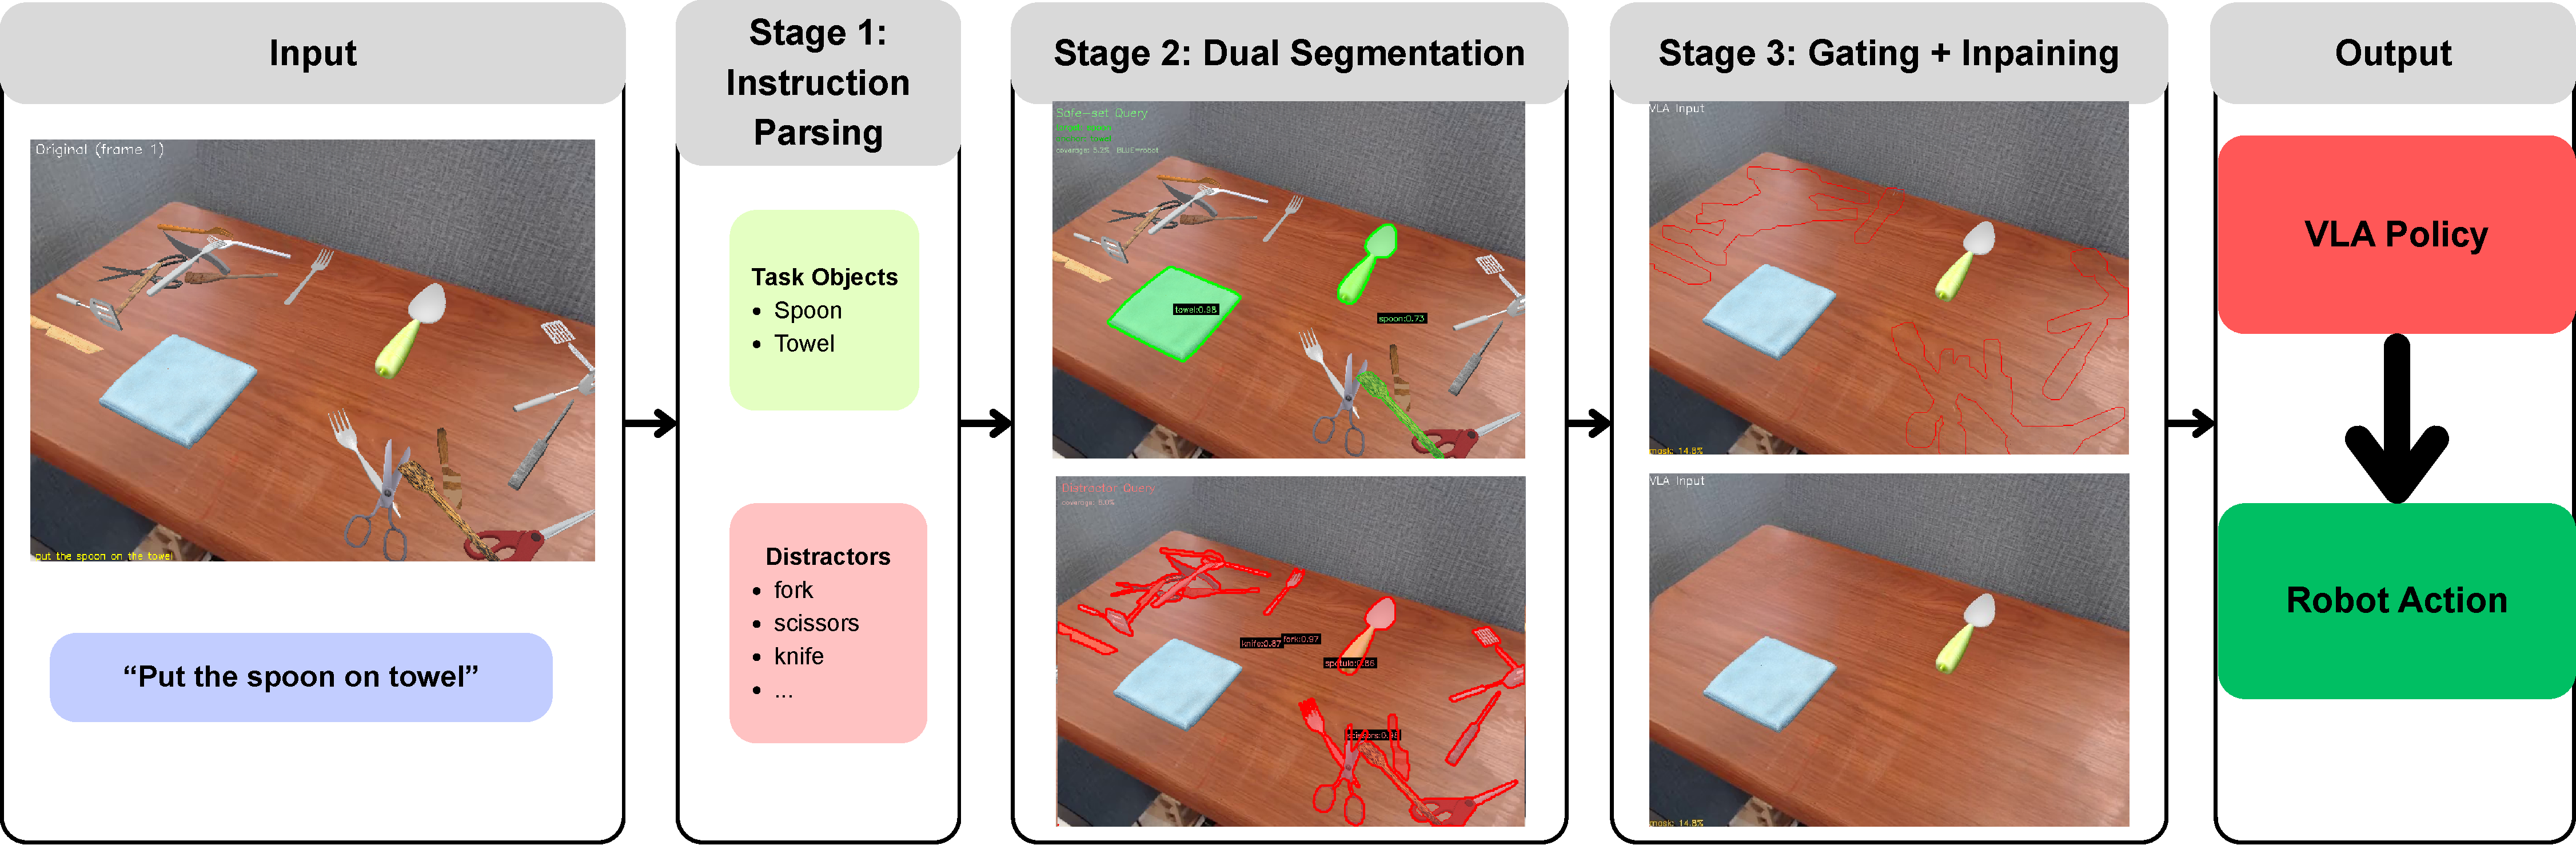
\includegraphics[width=0.78\textwidth]{figures/methodology.pdf}
    \caption{Overview of the CGVD pipeline. \textbf{Stage 1:} The language instruction is parsed to extract a safe set (target, anchor) and a distractor set. \textbf{Stage 2:} SAM~3 segments both sets independently, producing a safe-set mask and a distractor mask via dual-channel segmentation. \textbf{Stage 3:} Set-theoretic gating subtracts the safe-set mask from the distractor mask, and LaMa inpaints the resulting regions to produce a distilled observation passed to the VLA policy.}
    \label{fig:methodology}
\end{figure*}

Existing mitigations fall into three categories (\S II): observation-grounding methods such as OBEYED-VLA~\cite{obeyed} augment the VLA with a trained perception module that produces task-conditioned, object-centric, geometry-grounded observations, fine-tuning the policy on clean demonstrations; inference-time interventions such as BYOVLA~\cite{byovla} identify distractors with a VLM (an external GPT-4o dependency) and probe per-region sensitivity with multiple VLA forward passes, with threshold-based target protection; and training-time augmentation~\cite{rosie, genaug, nice} generates cluttered training data at the cost of retraining, without deployment-time guarantees.

To bridge this gap without the cost of retraining, we propose Concept-Gated Visual Distillation (CGVD): a model-agnostic inference framework that leverages modern vision foundation models~\cite{sam3} to selectively restructure visual observations before they reach the VLA policy. CGVD parses the task instruction to identify target and anchor objects, segments both distractors and task-relevant entities independently, and uses set-theoretic subtraction to produce a distractor mask from which the target is excluded \emph{conditional on correct safe-set segmentation}: the subtraction guarantees that no pixel segmented into the safe set is inpainted, but an object the segmenter fails to place in the safe set is not protected (\S\ref{sec:ablation}). Distractors are then replaced via inpainting~\cite{lama}, preserving the surrounding scene context.
%%%%%%%%%%%%%%%%%%%%%%%%%%%%%%%%%%%%%%%%%%%%%%%%%%%%%%%%%%%%%%%%%%%%%%%%%%%%%%%%


Our contributions are as follows:
\begin{itemize}
    \item \textbf{Concept-Gated Visual Distillation (CGVD):} We introduce a training-free, model-agnostic inference framework that selectively removes distractors from VLA observations via language-grounded segmentation and inpainting, while preserving scene context.

    \item \textbf{Interaction-Aware Masking Logic:} a set-theoretic cross-validation pipeline that overcomes the semantic confusion of open-set segmenters (which score prompts independently), penalizing false positives and spatially disambiguating true targets from confusable distractors.

    \item \textbf{Systematic clutter-density evaluation:}  We evaluate CGVD on two VLAs ($\pi_0$, GR00T) within the SimplerEnv benchmark over more than 20{,}000 episodes, comparing each policy with and without CGVD under matched seeds. CGVD prevents policy collapse under dense \emph{semantic} clutter---reaching 77.5\% success against the un-augmented policy's 43.0\% ($\pi_0$, \textit{put spoon on towel}, 18 semantic distractors; Table~\ref{tab:ablation})---and improves adherence to compositional attribute prompts, while \emph{underperforming} the baseline on a task where contextual clutter aids the policy (\S\ref{sec:main_results}). Comparisons are against the un-augmented policies, plus a measured head-to-head against a vocabulary-matched reimplementation of BYOVLA~\cite{byovla} at the headline condition (\S\ref{sec:byovla}).
\end{itemize}



\section{Related Work}

\subsection{Vision-Language-Action Models}
VLA models such as RT-2 \cite{rt2}, OpenVLA \cite{openvla}, and Octo \cite{octo} leverage internet-scale vision-language pre-training for remarkable zero-shot generalization, yet struggle with high-precision geometric grounding in cluttered scenes~\cite{distracted_robot}. We hypothesize that the static patch resolution of ViT backbones \cite{vit_analysis} and the absence of coarse-to-fine zooming \cite{c2f_q_attention} make such architectures susceptible to feature dilution \cite{distracted_robot}: background clutter competing with task-relevant signals for representational capacity.

\subsection{Vision Foundation Models for Robotic Perception}
Vision Foundation Models such as SAM~3 \cite{sam3} and GroundingDINO \cite{groundingdino} localize objects from free-form text; robotics has mostly used them to \textit{add} information---value maps \cite{voxposer}, semantic maps \cite{conceptfusion}, labeling \cite{robogen}, visual prompting \cite{RoboticVisualInstruction}. We invert the paradigm, suppressing task-irrelevant regions instead: an information bottleneck only in an informal, analogical sense~\cite{BC-IB}---no learned rate--distortion trade-off, just a hard pixel-space mask.

\subsection{Robustness via Training-Time Augmentation}
Clutter robustness has traditionally relied on domain randomization \cite{Tobin2017} and large-scale pre-training \cite{bridgedata, open_x_embodiment}, yet VLAs remain fragile to cluttered-scene shifts \cite{colosseum, robocasa}. Training-time augmentation generates cluttered or counterfactual data: ROSIE \cite{rosie}, GenAug \cite{genaug}, and NICE \cite{nice}, whose pixel-space \emph{scene surgery} is the closest prior to our core operation. CGVD performs a related pixel-space edit at \emph{inference} time on a frozen policy: no retraining, instruction-adaptive, but inheriting run-time perception risk.

\subsection{Inference-Time Attention Intervention}
Distracting Token Pruning (DTP) \cite{dtp} suppresses text-misaligned visual tokens in feature space; we conjecture such pruning struggles once distractor and target tokens are entangled by early self-attention, and instead intervene in pixel space, before tokenization. Unlike Visual Prompting \cite{RoboticVisualInstruction}, which adds information, we remove it. Two prior methods also operate on the observation: OBEYED-VLA \cite{obeyed} pairs the VLA with a \emph{trained} perception module producing task-conditioned, object-centric, geometry-grounded views and fine-tunes the policy on clean single-object demonstrations, whereas CGVD trains and fine-tunes nothing; BYOVLA \cite{byovla} intervenes at run time like CGVD, and \S\ref{sec:byovla} reports a measured comparison.

\section{Methodology}
\label{sec:methodology}
CGVD is a training-free, inference-time perception wrapper around any VLA policy (Fig.~\ref{fig:methodology}): given instruction $l$ and observation $o_t \in \mathbb{R}^{H \times W \times 3}$, a distillation function $\phi$ produces $\hat{o}_t = \phi(o_t, l)$ with distractors replaced by background, and the policy acts on $a_t = \pi(\hat{o}_t, l)$. Since $\phi$ touches only the observation interface, it is architecture-agnostic. The key insight: the instruction already specifies which objects matter, and CGVD uses this signal to gate visual content.

%--------------------------------------------------------------
\subsection{Concept-Gated Decomposition}
\label{sec:decomposition}

CGVD begins by parsing the language instruction $l$ to extract a target concept $c_{\text{tgt}}$ and an anchor concept $c_{\text{anc}}$. For instance, ``put spoon on towel'' yields $c_{\text{tgt}} = \texttt{spoon}$ and $c_{\text{anc}} = \texttt{towel}$. These concepts define two sets:
\begin{itemize}
    \item The \textbf{safe set} $\mathcal{S} = \{c_{\text{tgt}},\; c_{\text{anc}}\}$: entities that must remain visible. The robot arm is also always preserved, but it is handled through a separate proprioceptive channel (\S\ref{sec:inpainting}--\ref{sec:compositing}) rather than through the segmentation-based safe-set mask.
    \item The \textbf{distractor set} $\mathcal{D} = \{d_1, \ldots, d_K\}$: semantic categories to be treated as clutter (e.g., spatula, fork, knife).
\end{itemize}

The safe set is derived deterministically from the instruction. The distractor set is \emph{not}: it is an externally supplied vocabulary. In our experiments, $\mathcal{D}$ is re-derived at every episode reset from the category labels of the objects the evaluation protocol actually spawned in that episode (\S\ref{sec:setup})---i.e., CGVD receives the exact ground-truth clutter inventory, per episode. At deployment, $\mathcal{D}$ would have to be supplied by the integrator as a site-specific vocabulary or proposed by an external model. Where prior work uses an LLM to determine relevance~\cite{byovla}, our parsing is deterministic and needs no API \emph{in this closed-vocabulary setting}---a different point on a coverage-versus-cost trade-off, not a strict improvement. \S\ref{sec:ablation} measures the dependence: a generic site-level vocabulary recovers the oracle gain in full; a vocabulary that misses the clutter forfeits it.

%--------------------------------------------------------------
\subsection{Text-Prompted Instance Segmentation}
\label{sec:segmentation}
Both the safe set and distractor set are segmented from the observation using SAM~3~\cite{sam3}. The two sets produce independent mask channels:
\begin{align}
    M_{\text{dist}} &= \textstyle\bigcup_{d_k \in \mathcal{D}} \textsc{Seg}(o_t,\, d_k), \label{eq:distractor_mask} \\
    M_{\text{safe}} &= \textsc{Seg}(o_t,\, c_{\text{tgt}}) \,\cup\, \textsc{Seg}(o_t,\, c_{\text{anc}}), \label{eq:safe_mask}
\end{align}
where $\textsc{Seg}(o_t, c)$ denotes the union of all instance masks returned by SAM~3 for concept $c$ in observation $o_t$. An important computational optimization is that the vision encoder is executed only once for the initialization frame ($t=0$), with its masks reused across all frames of the episode.

%--------------------------------------------------------------
\subsection{Two-Layer Target Refinement}
\label{sec:refinement}
Open-set segmenters evaluate text prompts independently, so single-pass detection suffers semantic confusion: a spatula can yield high confidence for ``spoon.'' To ensure the true target survives distillation, we apply a two-layer refinement on the initial frame ($t{=}0$).

\textbf{Layer 1: Cross-Validation.} To penalize distractors, we compute a genuineness score $g(s_i)$ for each target instance $s_i$. This measures the confidence differential between its safe-set and distractor identities:
\begin{equation}
    g(s_i) = \sigma_{\text{safe}}(s_i) \;-\; \max_{\substack{d_j \in \mathcal{D} \\ \text{IoU}(s_i, d_j) > \eta}} \sigma_{\text{dist}}(d_j),
    \label{eq:genuineness}
\end{equation}
where $\sigma_{\text{safe}}$ and $\sigma_{\text{dist}}$ are object confidences, and $\eta$ is an IoU threshold ($\eta = 0.30$). When no distractor satisfies $\text{IoU}(s_i, d_j) > \eta$---the common case for an isolated target---the maximum is defined as $0$, so $g(s_i)$ reduces to $\sigma_{\text{safe}}(s_i)$. Genuine targets yield $g > 0$, while imposters yield $g < 0$. Negative values are explicitly preserved to actively penalize false positives in the next layer.

\textbf{Layer 2: Spatial Disambiguation.} Even after cross-validation, the target mask may contain fragmented artifacts or multiple disjoint physical objects. To isolate the correct entity, we evaluate each connected component $C_k$ using a composite score:
\begin{equation}
    \text{score}(C_k) = \bigl(1 + g^*(C_k)\bigr) \cdot \sigma^*(C_k).
    \label{eq:layer3}
\end{equation}
Here, $g^*(C_k)$ is maximum genuineness, and $\sigma^*(C_k)$ is peak safe-set confidence. These factors jointly favor genuine and high-confidence components. Only the top-scoring component is retained; the pipeline therefore assumes a \emph{single} target instance per scene (\S\ref{sec:limitations}).

For example, a spatula misidentified as ``spoon'' ($\sigma_{\text{safe}}{=}0.6$) but correctly detected as ``spatula'' ($\sigma_{\text{dist}}{=}0.9$) receives $g{=}{-}0.3$ and a penalized composite score $(1-0.3)\cdot 0.6 = 0.42$, letting the true spoon (high positive genuineness) outscore the imposter.



\subsection{Concept-Gated Mask Composition}
\label{sec:gating}
The refined masks are combined into a final inpainting mask via set-theoretic gating:
\begin{equation}
    M_{\text{inp}} = \text{dilate}(M_{\text{dist}},\, r_d) \;\setminus\; \text{dilate}(M_{\text{safe}},\, r_s),
    \label{eq:gating}
\end{equation}
where $r_d$ is a distractor dilation radius, and $r_s \geq r_d$ is a safe-set dilation radius that creates a protective buffer; the implementation enforces $r_s \geq r_d$ by construction, and both are 11\,px in our configuration. All masks are binarized with a threshold of $0.5$ before dilation to eliminate soft-value artifacts.

\subsection{Clean Scene Generation via Inpainting}
\label{sec:inpainting}
We generate a single clean scene---an image of the workspace with distractors removed---by applying LaMa \cite{lama}, a Fourier convolution-based inpainting model, to the initial frame. The inpainting mask is constructed as:
\begin{equation}
    M_{\text{lama}} = M_{\text{inp}} \;\cup\; \text{dilate}(M_{\text{robot}},\, r_e),
    \label{eq:inpaint_mask}
\end{equation}
where $M_{\text{robot}}$ is the robot mask (obtained as described in \S\ref{sec:compositing}) and $r_e$ is a robot dilation radius (20\,px). Including the robot region lets LaMa synthesize the background \emph{behind} the arm, so that the cached clean scene contains no stale robot pixels once the arm moves. A consequence is that scene content occluded by the arm at $t{=}0$ is synthesized rather than observed for the remainder of the episode (\S\ref{sec:limitations}). LaMa fills the masked regions with photorealistic background texture. The clean scene is computed once per episode and cached for all subsequent frames.

%--------------------------------------------------------------

\subsection{Temporally Consistent Compositing}
\label{sec:compositing}
At each timestep $t > 0$, the distilled observation is produced by alpha-blending the live camera frame with the cached clean scene:
\begin{equation}
    \hat{o}_t = \alpha \odot \hat{o}_{\text{clean}} + (1 - \alpha) \odot o_t,
    \label{eq:compositing}
\end{equation}
where the compositing mask $\alpha \in [0,1]^{H \times W}$ is computed \emph{once} at $t{=}0$ and held fixed: the binarized, safe-set-gated distractor mask is feathered with a Gaussian blur ($\sigma = 3.0$), clamped to $1$ in core distractor regions and $0$ in the (dilated) target region. So that inpainting artifacts never obscure the arm, robot pixels are overwritten onto the composite every step---the only per-frame operation. In simulation this robot mask comes from SimplerEnv's renderer segmentation buffer (per-link actor IDs): pixel-perfect, jitter-free, and \emph{simulation-privileged}; \S\ref{sec:ablation} measures the cost of substituting a per-frame SAM~3 prediction, and on hardware a forward-kinematics projection through the calibrated camera provides a deterministic, perception-free replacement.

Two properties should be stated explicitly. First, $\hat{o}_t$ is the \emph{only} visual input the policy receives. Second, the characteristic failure mode of observation editing is \emph{false-positive erasure}: an object misclassified as a distractor---or entering the workspace after $t{=}0$, where the fixed $\alpha$ can blend it toward the cached background---is removed from the policy's view while remaining in the world, and the arm can collide with what it cannot see. Our evaluation is therefore scoped to static workspaces with no human entry, a fixed camera, and a known clutter vocabulary.


\section{Experiments}
\label{sec:experiments}
We evaluate CGVD across two VLA architectures on tabletop manipulation tasks with controlled distractor injection. Our experiments address three questions: (1)~Does CGVD improve clutter robustness across different VLA architectures and tasks? (2)~How does performance scale with distractor density? (3)~How do individual CGVD components contribute at the operating point tested?

\subsection{Experimental Setup}
\label{sec:setup}
\textbf{Environment.} We evaluate in SimplerEnv~\cite{simplerenv}, whose real-to-sim correlation evidence supports \emph{policy-level} transfer of our findings. It does not bound CGVD's perception-level risk: SAM~3~\cite{sam3} and LaMa~\cite{lama} were trained on real imagery and are applied here to rendered frames---itself a domain shift---and two pipeline inputs are simulation-privileged (the renderer robot mask, \S\ref{sec:compositing}; the distractor vocabulary, \S\ref{sec:decomposition}). All conclusions are scoped to simulation (\S\ref{sec:limitations}).

All experiments use the WidowX robotic arm with a single fixed third-person camera, matching the Bridge dataset training setup. We test two Bridge dataset tasks: (1) \textit{put spoon on towel} and (2) \textit{put carrot on plate}.

\textbf{Policies.} $\pi_0$ refers to the open-source \texttt{open-pi-zero} reproduction of $\pi_0$~\cite{pi0}, Bridge checkpoint \texttt{bridge\_beta}\footnote{\texttt{github.com/allenzren/open-pi-zero}}; GR00T refers to \texttt{nvidia/GR00T-N1.6-bridge}~\cite{gr00t}\footnote{Ref.~\cite{gr00t} documents GR00T N1; the evaluated checkpoint is the N1.6 revision (different backbone and action head) --- see the NVIDIA model card at \texttt{huggingface.co/nvidia/GR00T-N1.6-bridge}.}. Both are frozen; CGVD touches only their image input.

\textbf{Distractors.} We introduce a three-way distractor taxonomy: \textit{Semantic} (high semantic proximity and shared visual characteristics with the target), \textit{Random} (no similarity), and \textit{Attribute} (same category and form, different physical properties); \cite{distracted_robot} documents the magnitude of clutter-induced degradation but uses a continuous clutter measure rather than these types. Assets come from RoboCasa~\cite{robocasa} and YCB~\cite{ycb}, placed collision-aware on a fixed 6\,cm grid (one object per cell); an unplaceable object falls back to a collision-free random position or is hidden off-scene---episodes are never dropped. The vocabulary $\mathcal{D}$ is re-derived per episode from the actually-spawned assets' category labels (\texttt{rc\_fork\_0} $\rightarrow$ ``fork''): it coincides exactly with each episode's injected inventory (\S\ref{sec:decomposition}).

\textbf{Protocol.} We report success rate (SR) via SimplerEnv's built-in per-task predicate over 60-step episodes: 20 episodes $\times$ 10 seeds per condition (200 episodes; the attribute study of Table~\ref{tab:combined_attribute_scaling} uses 5 seeds), with matched seeds between arms. Seed $s \in \{0,\dots,9\}$ seeds the Python/NumPy/PyTorch RNGs; episode $e$ uses canonical initial layout $(s{+}e) \bmod 24$ and distractor seed $10^4 s + e$, so both arms see identical initial states and clutter. Counts are sampled at $\{0, 4, 8, 10, 14, 18\}$; no episodes were excluded. We compare CGVD against the un-augmented policies throughout, and against a reimplementation of BYOVLA~\cite{byovla} at the headline condition (\S\ref{sec:byovla}). OBEYED-VLA's released code covers its perception module but not the action policy or robot interface, so an end-to-end comparison was infeasible; DTP's~\cite{dtp} only advertised release is an anonymized review-time repository that has since expired.

\textbf{Analysis.} We report episode-level mean success rates with, as dispersion, the SD of the 10 per-seed rates; differences carry 95\% CIs from the per-seed paired deltas ($t_9$). Episode-level clustering by seed is negligible (one-way ICC across all arms: median $-0.02$, max $0.06$). The headline contrast---$\pi_0$, \textit{put spoon on towel}, 18 semantic distractors---is the single confirmatory comparison ($\Delta = +34.5$\,pp, 95\% CI $[+20.8, +48.2]$, paired $t$ $p = 3{\times}10^{-4}$; Wilcoxon $p = 0.002$); all other contrasts are exploratory and unadjusted, and deltas whose CI contains zero are within run-to-run noise. The 0-distractor cells are shared between the semantic and random conditions (physically identical). The one condition executed twice end-to-end ($\pi_0$, \textit{carrot}, random, 18) differed between batches by 3.0\,pp (baseline) and 0.5\,pp (CGVD), a direct run-to-run replication estimate.

\textbf{Implementation.} All CGVD parameters, held fixed across every reported experiment: SAM~3 checkpoint \texttt{facebook/sam3}; LaMa big-lama (\texttt{simple-lama-inpainting}); confidence thresholds 0.30 (safe set) and 0.20 (distractors); $\eta = 0.30$; $r_d = r_s = 11$\,px; $r_e = 20$\,px; compositing $\sigma = 3.0$; mask binarization 0.5; minimum connected component 50\,px; one warm-up frame; clean scene cached once per episode, never refreshed; SAM~3 prompts are the instruction's noun phrases and the category labels of $\mathcal{D}$. Values were selected on small pilot rollouts (primarily of the spoon task) during development and frozen before any reported evaluation run was executed (verified from version-control history). Code, configuration, and evaluation scripts are available at \texttt{github.com/awd1779/pi0}.

%%% %%% %%% %%% %%% chart for SR %%% %%% %%% %%% %%% %%% %%%
\begin{figure*}[t]
  \centering
  
\includegraphics[width=0.92\textwidth]{figures/distractor_scaling.pdf}
    \caption{Success rate vs.\ distractor count. \textbf{Left:} semantic; \textbf{right:} random distractors. \textbf{Top:} \textit{put spoon on towel}; \textbf{bottom:} \textit{put carrot on plate}. Dashed: baseline VLA; solid: +CGVD; colors denote architectures. Each point is the mean over 200 rollouts (20 episodes $\times$ 10 matched seeds) at counts $\{0, 4, 8, 10, 14, 18\}$ (19{,}200 episodes total); 0-distractor points are shared between panels. Numeric values with dispersion and CIs: Table~\ref{tab:main_numeric}.}
  \label{fig:scaling}
\end{figure*}
%%% %%% %%% %%% %%% %%% %%% %%% %%% %%% %%% %%% %%% %%% %%%

% AUTO-GENERATED by analysis/phase2_analysis.py — do not edit by hand.
% Mean success rate (%) ± SD across the 10 matched seeds (20 episodes/seed).
\begin{table*}[t]
\centering
\caption{\textbf{Main results (numeric).} Success rate (\%), mean $\pm$ SD over 10 matched seeds (200 episodes/cell); $\Delta$ with 95\% CI from per-seed paired deltas ($t_9$), bold when the CI excludes zero.}
\label{tab:main_numeric}
\renewcommand{\arraystretch}{1.0}
\resizebox{\textwidth}{!}{%
\begin{tabular}{llcccccccccccc}
\hline
 & & \multicolumn{6}{c}{\textbf{Semantic distractors}} & \multicolumn{6}{c}{\textbf{Random distractors}} \\
\cline{3-8}\cline{9-14}
 & & \multicolumn{3}{c}{$\pi_0$} & \multicolumn{3}{c}{GR00T} & \multicolumn{3}{c}{$\pi_0$} & \multicolumn{3}{c}{GR00T} \\
\textbf{Task} & \textbf{\#D} & base & +CGVD & $\Delta$ [95\% CI] & base & +CGVD & $\Delta$ [95\% CI] & base & +CGVD & $\Delta$ [95\% CI] & base & +CGVD & $\Delta$ [95\% CI] \\
\hline
\textit{spoon on towel} & 0 & 82.0 & 85.0 & +3.0 [-5.6,+11.6] & 49.0 & 51.0 & +2.0 [-6.1,+10.1] & 82.0 & 85.0 & +3.0 [-5.6,+11.6] & 49.0 & 51.0 & +2.0 [-6.1,+10.1] \\
 & 4 & 59.0 & 73.0 & \textbf{+14.0 [+5.4,+22.6]} & 47.5 & 46.0 & -1.5 [-8.7,+5.7] & 70.5 & 78.0 & +7.5 [-0.8,+15.8] & 48.0 & 48.0 & +0.0 [-7.0,+7.0] \\
 & 8 & 51.0 & 73.5 & \textbf{+22.5 [+10.7,+34.3]} & 28.5 & 41.0 & \textbf{+12.5 [+6.4,+18.6]} & 62.5 & 74.0 & \textbf{+11.5 [+1.7,+21.3]} & 44.0 & 43.5 & -0.5 [-12.5,+11.5] \\
 & 10 & 49.0 & 72.5 & \textbf{+23.5 [+12.8,+34.2]} & 29.5 & 43.0 & \textbf{+13.5 [+6.1,+20.9]} & 60.0 & 78.5 & \textbf{+18.5 [+10.2,+26.8]} & 41.0 & 47.0 & +6.0 [-3.0,+15.0] \\
 & 14 & 52.5 & 75.5 & \textbf{+23.0 [+14.7,+31.3]} & 30.0 & 41.0 & \textbf{+11.0 [+3.3,+18.7]} & 64.5 & 77.5 & \textbf{+13.0 [+1.7,+24.3]} & 33.0 & 42.0 & +9.0 [-0.9,+18.9] \\
 & 18 & 43.0 & 77.5 & \textbf{+34.5 [+20.8,+48.2]} & 31.0 & 43.5 & \textbf{+12.5 [+4.0,+21.0]} & 57.5 & 70.5 & \textbf{+13.0 [+2.0,+24.0]} & 28.0 & 45.0 & \textbf{+17.0 [+7.6,+26.4]} \\
\hline
\textit{carrot on plate} & 0 & 58.5 & 54.5 & -4.0 [-11.7,+3.7] & 32.0 & 28.0 & -4.0 [-12.2,+4.2] & 58.5 & 54.5 & -4.0 [-11.7,+3.7] & 32.0 & 28.0 & -4.0 [-12.1,+4.1] \\
 & 4 & 57.5 & 52.5 & -5.0 [-11.5,+1.5] & 41.5 & 32.0 & \textbf{-9.5 [-12.1,-6.9]} & 56.0 & 53.0 & -3.0 [-10.8,+4.8] & 36.5 & 30.0 & -6.5 [-16.5,+3.5] \\
 & 8 & 62.0 & 53.0 & -9.0 [-21.1,+3.1] & 42.5 & 31.0 & \textbf{-11.5 [-17.1,-5.9]} & 55.0 & 52.5 & -2.5 [-10.8,+5.8] & 43.0 & 28.5 & \textbf{-14.5 [-21.1,-7.9]} \\
 & 10 & 61.5 & 53.5 & \textbf{-8.0 [-15.0,-1.0]} & 42.5 & 29.0 & \textbf{-13.5 [-20.7,-6.3]} & 56.0 & 55.0 & -1.0 [-10.7,+8.7] & 40.0 & 28.5 & \textbf{-11.5 [-18.7,-4.3]} \\
 & 14 & 58.5 & 51.5 & -7.0 [-17.4,+3.4] & 32.0 & 27.5 & -4.5 [-9.7,+0.7] & 53.5 & 52.0 & -1.5 [-13.8,+10.8] & 39.0 & 37.5 & -1.5 [-9.2,+6.2] \\
 & 18 & 56.0 & 47.0 & \textbf{-9.0 [-17.7,-0.3]} & 32.0 & 28.5 & -3.5 [-10.0,+3.0] & 49.5 & 54.0 & +4.5 [-6.9,+15.9] & 38.0 & 41.0 & +3.0 [-3.6,+9.6] \\
\hline
\end{tabular}%
}
\end{table*}


\subsection{Main Results}
\label{sec:main_results}
Figure~\ref{fig:scaling} plots success rate against distractor count (0--18); Table~\ref{tab:main_numeric} reports the numbers with per-seed dispersion and paired CIs. Trends differ sharply by task and clutter type.

On \textit{put spoon on towel}, baseline performance degrades precipitously under semantically confusing clutter, and CGVD prevents this collapse: $\pi_0$ gains $+14.0$ to $+34.5$\,pp for $n \geq 4$ and GR00T gains $+11.0$ to $+13.5$\,pp for $n \geq 8$, with every paired CI excluding zero. The gap widens with density: the per-seed slope of the CGVD$-$baseline difference is $+1.54$\,pp per distractor for $\pi_0$ ($t(9){=}5.54$, $p{<}0.001$) and $+0.74$ for GR00T ($t(9){=}2.77$, $p{=}0.02$). Random clutter shows the same direction at high density ($\pi_0$: $+13.0$ $[+2.0, +24.0]$; GR00T: $+17.0$ $[+7.6, +26.4]$ at 18 distractors).

Conversely, on \textit{put carrot on plate} the baseline policies \emph{improve} at moderate densities before degrading---plausibly because moderate contextual clutter better matches the object-rich scenes of their pre-training distributions, providing visual anchors.

Here CGVD never significantly outperforms the baseline and significantly underperforms it at several densities: $\pi_0$'s semantic deltas span $-4.0$ to $-9.0$\,pp (CIs exclude zero at $n{=}10, 18$), and GR00T loses $-9.5$ to $-14.5$\,pp at moderate densities under both clutter types. When a task benefits from contextual clutter, masking deprives the VLA of useful anchors, and inpainting artifacts can disrupt spatial geometry: the intervention is \emph{task- and distractor-type-conditional}, not universally beneficial.

Qualitative attention visualizations consistent with the working hypothesis---extracted by hooking every self-attention layer of $\pi_0$'s PaliGemma backbone and averaging final-query-token attention over the 256 SigLIP visual tokens across layers and heads---are provided in the code repository. We emphasize that such visualizations are entailed by the intervention itself (removing a distractor's pixels removes attention on them) and that no attention statistic is measured in this paper; alternative explanations---such as CGVD restoring the observation toward the clutter-sparse Bridge training distribution, or simply deleting the wrong-grasp option---are consistent with our data and are not ruled out. Indeed, the mean-color-fill ablation (\S\ref{sec:ablation}), in which removing the \emph{same} semantic content with a cruder fill forfeits most of the gain, indicates that fill appearance, not distractor semantics alone, carries a large share of the effect.

\subsection{Fine-Grained Semantic Grounding}
\label{sec:attribute}
The precision-reasoning gap is most acute when distractors share the target's semantic class but differ in attributes: complex queries like ``Put spoon with green handle on towel'' are often reduced to a bag-of-words, entangling the target with fully green objects or dropping modifiers. We use the \textit{Attribute} type (\S\ref{sec:setup}): a green-handled spoon target among same-category spoons differing in color or material. We evaluate the baseline and CGVD across 0--4 attribute distractors using two prompt structures: Simple (``Put green spoon on towel'') and Complex (``Put spoon with green handle on towel''). CGVD receives the same instruction as the policy; its SAM~3 target prompt is the instruction's attribute phrase (``green spoon'' / ``spoon with green handle''). Note the coverage asymmetry: the attribute type is evaluated on one task with $\pi_0$ only, at 0--4 distractors, whereas Fig.~\ref{fig:scaling} covers the semantic and random types on both tasks and both policies at 0--18 distractors. Generality claims for attribute clutter are correspondingly scoped.

Table~\ref{tab:combined_attribute_scaling} reveals a two-sided dependence on descriptive density. The baseline degrades mildly with clutter under simple adjective-noun prompts (87.0\% $\rightarrow$ 75.0\%) but collapses on compositional queries (86.0\% $\rightarrow$ 57.0\%)---the bag-of-words brittleness. For CGVD, the complex prompt is what unlocks the benefit: it holds a stable floor under the compositional query (73.0\% at 4 distractors, $\Delta = +16.0$, the one delta whose CI excludes zero) because SAM~3 exploits the rich attribute phrase to isolate the correct instance, whereas under the \emph{simple} prompt CGVD provides no reliable benefit (deltas $-5.0$ to $+3.0$, all within noise): ``green spoon'' gives the segmenter too little signal to separate the target from attribute-conflicting spoons. The bottleneck is the segmentation prompt: supplying the scene-informed phrase ``spoon with green handle'' under the simple instruction restores large gains (87.0/82.0/83.0 at 2--4 distractors vs.\ 79.0--70.0), but that phrasing encodes scene knowledge not derivable from the instruction, so the instruction-consistent numbers are primary. CGVD converts descriptive density into robustness; it does not rescue a prompt that lacks it. Given the 5-seed sample, per-cell values here are descriptive.

% AUTO-GENERATED by analysis/phase2_analysis.py — do not edit by hand.
\begin{table}[!t]
\centering
\caption{\textbf{Attribute Distractor Sensitivity.} Success rates on \textit{put spoon on towel} with attribute distractors ($\pi_0$ only), 100 episodes per cell (5 matched seeds $\times$ 20 episodes). $\Delta$ carries a 95\% CI from per-seed paired deltas; bold marks deltas whose CI excludes zero. Deltas whose CI contains zero are within run-to-run noise.}
\label{tab:combined_attribute_scaling}
\renewcommand{\arraystretch}{1.2}
\resizebox{\columnwidth}{!}{%
\begin{tabular}{l ccc ccc}
\hline
& \multicolumn{3}{c}{\textbf{Simple Prompt}}
& \multicolumn{3}{c}{\textbf{Complex Prompt}} \\
\cline{2-4} \cline{5-7}
\textbf{\# Distractors}
  & \textbf{$\pi_0$} & \textbf{+CGVD} & \textbf{$\Delta$ [95\% CI]}
  & \textbf{$\pi_0$} & \textbf{+CGVD} & \textbf{$\Delta$ [95\% CI]} \\
\hline
0 & 87.0 & 85.0 & -2.0 [-13.3,+9.3] & 86.0 & 87.0 & +1.0 [-5.8,+7.8] \\
1 & 79.0 & 80.0 & +1.0 [-7.1,+9.1] & 74.0 & 69.0 & -5.0 [-26.9,+16.9] \\
2 & 76.0 & 79.0 & +3.0 [-14.9,+20.9] & 69.0 & 77.0 & +8.0 [-9.9,+25.9] \\
3 & 77.0 & 75.0 & -2.0 [-20.4,+16.4] & 64.0 & 74.0 & +10.0 [-7.6,+27.6] \\
4 & 75.0 & 70.0 & -5.0 [-24.6,+14.6] & 57.0 & 73.0 & \textbf{+16.0 [+1.2,+30.8]} \\
\hline
\end{tabular}%
}
\end{table}


\begin{table}[t!]
\centering
\caption{ \textbf{Ablation study} ($\pi_0$, \textit{put spoon on towel}, 18 semantic distractors; 200 episodes/row). Rows remove or substitute one component. SR: mean $\pm$ SD over per-seed rates; $\Delta$ vs.\ full pipeline with 95\% CI from paired deltas. Baseline/full rows reuse the Fig.~\ref{fig:scaling} runs; the robot-mask effect is not distinguishable from zero.}
\label{tab:ablation}
\begin{tabular}{lcc}
\hline
\textbf{Configuration} & \textbf{SR (\%)} & \textbf{$\Delta$ [95\% CI]} \\
\hline
Baseline (no CGVD)        & 43.0\,$\pm$\,16.0 & $-34.5$ $[-48.2, -20.8]$ \\
CGVD (full pipeline)               & \textbf{77.5}\,$\pm$\,6.3 & --- \\
\quad LaMa $\rightarrow$ mean-color fill   & 56.5\,$\pm$\,16.0 & $-21.0$ $[-35.3, -6.7]$ \\
\quad -- Two-layer target refinement & 65.0\,$\pm$\,8.8 & $-12.5$ $[-20.3, -4.7]$ \\
\quad -- Robot mask protection     & 73.0\,$\pm$\,7.1 & $-4.5$ $[-10.4, +1.4]$ \\
\hline
\end{tabular}
\end{table}

\subsection{Ablation Studies}
\label{sec:ablation}
We ablate the pipeline at a single operating point---\textit{put spoon on towel}, $\pi_0$, 18 semantic distractors (Table~\ref{tab:ablation}); $\pi_0$'s higher success rates provide headroom to resolve component contributions. The attributions are claims about this operating point only: \S\ref{sec:main_results} shows the pipeline's net effect reverses in other regimes.

Removing the Two-Layer Target Refinement reduces SR from 77.5\% to 65.0\%: without cross-validation, genuine targets are erroneously inpainted out of the scene---CGVD's own protection fails, which is why we call it conditional (\S\ref{sec:decomposition}). To quantify the residual failure rate of the \emph{full} pipeline, we audited a fresh 200-episode re-execution of the headline condition against the renderer's ground-truth target mask: the final inpainting mask overlapped the target at $t{=}0$ in 4 of 200 episodes (2.0\%), and in all four cases the target was erased essentially completely. The protection is therefore strong but probabilistic in practice, differing from sensitivity-probe approaches in failure \emph{rate}, not failure \emph{mode}. (This re-execution also provides a replication of the headline cell: 76.0\% vs.\ the original 77.5\%.) Substituting a mean-color fill for LaMa incurs the largest single drop (56.5\%) despite identical masks and removed content; we hypothesize (unmeasured) that the stark boundaries act like out-of-distribution patches to the ViT backbone. Notably, a majority of the gain at this operating point thus depends on \emph{how} regions are filled, not on removal alone. Finally, removing Robot Mask Protection reduces SR to 73.0\%; this $-4.5$\,pp effect is not statistically distinguishable from zero at our sample size (95\% CI $[-10.4, +1.4]$), so we treat robot-mask protection as qualitatively motivated---without it, the compositing mask occasionally and visibly occludes the robot arm---rather than as a measured gain.

\textbf{Deployable robot mask.} To measure the cost of the renderer mask's simulation privilege, we additionally ran the full pipeline with a \emph{per-frame SAM~3 prediction} (prompt ``robot arm'') replacing the renderer mask, on the same seeds. Success is statistically unchanged---74.0\% vs.\ 76.0\% for a ground-truth-mask re-execution (paired $\Delta = -2.0$\,pp, 95\% CI $[-11.3, +7.3]$)---but the deployable path costs $240.7 \pm 1.9$\,ms per frame (dropping the control rate to ${\approx}1.7$\,Hz) and SAM~3 returns \emph{no} robot detection in 20.1\% of frames, falling back to the previous mask. The simulation privilege is thus primarily a latency-and-reliability privilege rather than an accuracy one, and forward-kinematics projection (\S\ref{sec:compositing}) remains the sensible hardware path.

\textbf{Vocabulary sensitivity.} Since $\mathcal{D}$ coincides with the injected inventory (\S\ref{sec:decomposition}), we re-ran the headline condition (same seeds, CGVD arm) with two \emph{frozen} vocabularies to measure that privilege. With a vocabulary that misses the injected clutter ($\mathcal{D} = \{$ladle, whisk, bowl, cup$\}$), success collapses to 45.5\%---statistically indistinguishable from the 43.0\% baseline (paired $\Delta$ vs.\ baseline $+2.5$, 95\% CI $[-6.6, +11.6]$). With a \emph{generic} 12-category tabletop vocabulary not derived from the injection list (utensils and tableware), success is 76.5\%---statistically indistinguishable from the oracle vocabulary ($\Delta$ vs.\ oracle re-execution $+0.5$ $[-4.7, +5.7]$; vs.\ baseline $+33.5$ $[+22.3, +44.7]$). CGVD's benefit therefore requires vocabulary \emph{coverage} of the clutter, but not knowledge of the exact inventory: a plausible site-level vocabulary recovers the oracle-level gain in full, while a vocabulary miss forfeits it entirely.



\subsection{Comparison with a Run-Time Intervention Baseline}
\label{sec:byovla}
We compare CGVD against BYOVLA~\cite{byovla}, the closest prior run-time observation intervention, at the headline condition (same 10 matched seeds, 200 episodes), reimplementing it from its reference code with three substitutions chosen to remove confounds: GPT-4o replaced by the \emph{same} closed vocabulary $\mathcal{D}$ CGVD receives, GroundingDINO+SAM2 by SAM~3 (shared with CGVD), and Octo's fixed-key stochastic probe by fixed-seed $\pi_0$ forward passes. The mechanism is kept faithful: per-object Gaussian-blur perturbation (random kernel 15--30), translation-only action deltas with the reference threshold (0.002\,m, same physical units), sensitive-region inpainting (dilation 10), re-run before every action chunk. The probe demonstrably discriminates here (mean 2.0 of 32.1 candidate regions flagged per chunk, range 0--16).

The result is one-sided: BYOVLA reaches 32.5\%---below the 43.0\% baseline ($\Delta = -10.5$, 95\% CI $[-25.7, +4.7]$) and far below CGVD's 77.5\% (paired $\Delta = -45.0$ $[-56.4, -33.6]$)---while each intervention costs $11.3 \pm 2.0$\,s (${\sim}33$ policy forwards), roughly $34\times$ CGVD's \emph{total} per-step cost. We see two causes: per-chunk re-segmentation and re-inpainting makes the background flicker across chunks (Table~\ref{tab:ablation}'s mean-color-fill row shows the policy is highly sensitive to fill appearance---the instability CGVD's cached clean plate avoids), and at 18 distractors the conservative threshold leaves most clutter in view. Two caveats: this is our reimplementation, not the authors' system, and 18 dense distractors is well outside BYOVLA's original regime (a real robot, a handful of distractors); we did not tune its threshold. The fair conclusion is that per-chunk probe-and-inpaint does not scale to dense clutter, not that the method fails in its intended regime.

\subsection{Latency Analysis}
\label{sec:latency}
CGVD concentrates its expensive operations (SAM~3, LaMa) on the initialization frame ($t=0$); for $t>0$ the system performs image compositing against the cached clean scene. Table~\ref{tab:latency} reports timing measured on an NVIDIA A10G (23\,GB) across the evaluation runs. The policy forward pass is unaffected ($318.1 \pm 6.6$\,ms baseline vs.\ $318.5 \pm 5.5$\,ms under CGVD), and per-frame compositing adds $15.6 \pm 0.4$\,ms, i.e.\ ${\approx}{+}5\%$ per control step (${\approx}3.14 \rightarrow 3.00$\,Hz). Initialization is a one-off per-episode cost that grows with the number of segmentation prompts: $0.68 \pm 0.29$\,s in the attribute scenes ($\leq$5 prompts) and ${\approx}3.3$\,s in the 18-distractor scenes (derived from episode wall time), delaying the first action of each episode. The overhead is modest for the quasi-static tabletop tasks evaluated here; the startup delay remains a real cost for time-critical settings.

 \begin{table}[htbp]
  \centering
  \caption{\textbf{System Latency}, measured on an NVIDIA A10G across the evaluation runs (mean $\pm$ SD over episodes; $n$ in parentheses). CGVD concentrates segmentation and inpainting at $t{=}0$; runtime compositing adds ${\approx}5\%$ per step.}
  \label{tab:latency}
  \resizebox{\columnwidth}{!}{%
  \begin{tabular}{lc}
  \hline
  \textbf{Quantity} & \textbf{Measured} \\
  \hline
  Policy forward / step, baseline & $318.1 \pm 6.6$\,ms \,(500 ep.) \\
  Policy forward / step, with CGVD & $318.5 \pm 5.5$\,ms \,(1{,}100 ep.) \\
  CGVD compositing / frame ($t>0$) & $15.6 \pm 0.4$\,ms \,(500 ep.) \\
  Initialization ($t=0$), $\leq$5 prompts & $0.68 \pm 0.29$\,s \,(500 ep.) \\
  Initialization ($t=0$), 18-distractor scenes & ${\approx}3.3$\,s (wall-time derived) \\
  \hline
  \end{tabular}%
  }
  \end{table}



\section{Limitations}
\label{sec:limitations}

CGVD's validity envelope is defined by the following assumptions and scope limits.

\textbf{Static scene.} The clean scene is cached at $t{=}0$ and $\alpha$ is fixed (\S\ref{sec:compositing}). A moved distractor desynchronizes the cache; worse, an object \emph{entering} the workspace after $t{=}0$ can be blended toward the cached background and hidden from the policy while physically present---a hazard, not merely an accuracy loss, outside access-controlled workspaces. Continuous re-segmentation would remove this assumption but is prohibitive at control rate.

\textbf{Contextually informative clutter.} On \textit{put carrot on plate} CGVD never outperforms the baseline and significantly underperforms it at several densities (up to $-14.5$\,pp for GR00T; \S\ref{sec:main_results}): the intervention is task- and distractor-type-conditional, and deciding \emph{when} to distill is open future work.

\textbf{Simulation-only evaluation and privileged inputs.} No real-robot experiment is reported, and two inputs are simulation-privileged: the renderer robot mask and the per-episode distractor inventory $\mathcal{D}$. SAM~3 recall over $\mathcal{D}$ and LaMa fill fidelity on real textured scenes (the largest single factor in Table~\ref{tab:ablation}) are unvalidated on hardware; the deployable per-frame SAM~3 robot mask is measured in simulation only (\S\ref{sec:ablation}), and FK projection on hardware is untested.

\textbf{Single target instance.} Layer 2 retains only the top-scoring component (\S\ref{sec:refinement}); a scene with two genuine target instances would have one inpainted away.

\textbf{Occlusion fabrication and in-flight blending.} Whatever the arm occluded at $t{=}0$ is synthesized, not observed, in the cached scene (Eq.~\ref{eq:inpaint_mask}); and since $\alpha$ protects the target only at its $t{=}0$ location, the \emph{moving} target overlaps previously inpainted regions by ${>}10\%$ in 35\% of audited episodes, exposing the grasped object to partial blending. Finally, initialization delays each episode's first action by $0.7$--$3.3$\,s (Table~\ref{tab:latency}).

\section{Conclusion}
We introduced Concept-Gated Visual Distillation (CGVD), a training-free inference framework that mitigates the Precision-Reasoning Gap in VLA models via language-grounded segmentation and inpainting, without architectural modification. Across more than 20{,}000 SimplerEnv episodes with $\pi_0$ and GR00T, CGVD prevents performance collapse under dense semantic clutter and improves adherence to compositional attribute prompts, relative to the un-augmented policies; at the headline condition it outperforms a vocabulary-matched BYOVLA reimplementation by 45\,pp at a small fraction of its per-step cost. The benefit is conditional: where contextual clutter aids the policy, CGVD never outperforms and often significantly underperforms the baseline. Bounded by static-background and closed-vocabulary assumptions, these results position inference-time visual distillation as a practical defense against semantically confusable clutter in static scenes. Future work: real-time mask updating, intrusion detection over compositing regions, open-vocabulary $\mathcal{D}$, and criteria for when to distill.

%\addtolength{\textheight}{-12cm}   % This command serves to balance the column lengths
                                  % on the last page of the document manually. It shortens
                                  % the textheight of the last page by a suitable amount.
                                  % This command does not take effect until the next page
                                  % so it should come on the page before the last. Make
                                  % sure that you do not shorten the textheight too much.

%%%%%%%%%%%%%%%%%%%%%%%%%%%%%%%%%%%%%%%%%%%%%%%%%%%%%%%%%%%%%%%%%%%%%%%%%%%%%%%%

% Using BibTeX for the references
{\footnotesize
\bibliographystyle{IEEEtran}
\bibliography{references}
}

\end{document}
